% Options for packages loaded elsewhere
\PassOptionsToPackage{unicode}{hyperref}
\PassOptionsToPackage{hyphens}{url}
%
\documentclass[
]{article}
\usepackage{amsmath,amssymb}
\usepackage{iftex}
\ifPDFTeX
  \usepackage[T1]{fontenc}
  \usepackage[utf8]{inputenc}
  \usepackage{textcomp} % provide euro and other symbols
\else % if luatex or xetex
  \usepackage{unicode-math} % this also loads fontspec
  \defaultfontfeatures{Scale=MatchLowercase}
  \defaultfontfeatures[\rmfamily]{Ligatures=TeX,Scale=1}
\fi
\usepackage{lmodern}
\ifPDFTeX\else
  % xetex/luatex font selection
\fi
% Use upquote if available, for straight quotes in verbatim environments
\IfFileExists{upquote.sty}{\usepackage{upquote}}{}
\IfFileExists{microtype.sty}{% use microtype if available
  \usepackage[]{microtype}
  \UseMicrotypeSet[protrusion]{basicmath} % disable protrusion for tt fonts
}{}
\makeatletter
\@ifundefined{KOMAClassName}{% if non-KOMA class
  \IfFileExists{parskip.sty}{%
    \usepackage{parskip}
  }{% else
    \setlength{\parindent}{0pt}
    \setlength{\parskip}{6pt plus 2pt minus 1pt}}
}{% if KOMA class
  \KOMAoptions{parskip=half}}
\makeatother
\usepackage{xcolor}
\usepackage[margin=1in]{geometry}
\usepackage{graphicx}
\makeatletter
\def\maxwidth{\ifdim\Gin@nat@width>\linewidth\linewidth\else\Gin@nat@width\fi}
\def\maxheight{\ifdim\Gin@nat@height>\textheight\textheight\else\Gin@nat@height\fi}
\makeatother
% Scale images if necessary, so that they will not overflow the page
% margins by default, and it is still possible to overwrite the defaults
% using explicit options in \includegraphics[width, height, ...]{}
\setkeys{Gin}{width=\maxwidth,height=\maxheight,keepaspectratio}
% Set default figure placement to htbp
\makeatletter
\def\fps@figure{htbp}
\makeatother
\setlength{\emergencystretch}{3em} % prevent overfull lines
\providecommand{\tightlist}{%
  \setlength{\itemsep}{0pt}\setlength{\parskip}{0pt}}
\setcounter{secnumdepth}{-\maxdimen} % remove section numbering
\ifLuaTeX
  \usepackage{selnolig}  % disable illegal ligatures
\fi
\usepackage{bookmark}
\IfFileExists{xurl.sty}{\usepackage{xurl}}{} % add URL line breaks if available
\urlstyle{same}
\hypersetup{
  hidelinks,
  pdfcreator={LaTeX via pandoc}}

\author{}
\date{\vspace{-2.5em}}

\begin{document}

\subsection{Inhaltsverzeichnis}\label{inhaltsverzeichnis}

\begin{itemize}
\tightlist
\item
  \hyperref[A_1_Kinoklub]{1 Kinoklub}
\item
  \hyperref[A_2_Installation]{2 Installation}
\item
  \hyperref[A_3_Gitux5cux2520Passwortux5cux2520ux2fux5cux2520Personalux5cux2520Accessux5cux2520Tokenux5cux2520ux28PATux29]{3
  Git Passwort / Personal Access Token (PAT)}
\item
  \hyperref[A_4_Datensuxe4tze]{4 Datensätze}

  \begin{itemize}
  \tightlist
  \item
    \hyperref[A_4.1_Advance-Tickets]{4.1 Advance-Tickets}

    \begin{itemize}
    \tightlist
    \item
      \hyperref[A_4.1.1_Eintritte]{4.1.1 Eintritte}
    \item
      \hyperref[A_4.1.2_Kiosk]{4.1.2 Kiosk}
    \item
      \hyperref[A_4.1.3_Shows]{4.1.3 Shows}
    \end{itemize}
  \item
    \hyperref[A_4.2_Excelux5cux2520Dateien]{4.2 Excel Dateien}

    \begin{itemize}
    \tightlist
    \item
      \hyperref[A_4.2.1_Einkaufspreise]{4.2.1 Einkaufspreise}
    \item
      \hyperref[A_4.2.2_Spezialpreiseux5cux2520Kiosk]{4.2.2
      Spezialpreise Kiosk}
    \item
      \hyperref[A_4.2.3_Verleiherabgaben]{4.2.3 Verleiherabgaben}
    \item
      \hyperref[A_4.2.4_Einnahmenux5cux2520undux5cux2520Ausgaben]{4.2.4
      Einnahmen und Ausgaben}
    \end{itemize}
  \end{itemize}
\item
  \hyperref[A_5_Scriptux5cux2520Konfiguration]{5 Script Konfiguration}

  \begin{itemize}
  \tightlist
  \item
    \hyperref[A_5.1_Abrechnungux5cux2520fuxfcrux5cux2520Filmvorfuxfchrungen]{5.1
    Abrechnung für Filmvorführungen}
  \item
    \hyperref[A_5.2_Inhaltsverzeichnisse]{5.2 Inhaltsverzeichnisse}
  \item
    \hyperref[A_5.3_Mehrwertsteuersatz]{5.3 Mehrwertsteuersatz}
  \item
    \hyperref[A_5.4_Platzkategorienux5cux2520ohneux5cux2520Umsatzux5cux2520dieux5cux2520dennochux5cux2520abgerechnetux5cux2520werdenux5cux2520muxfcssen.]{5.4
    Platzkategorien ohne Umsatz die dennoch abgerechnet werden müssen.}
  \item
    \hyperref[A_5.5_Ausgabeformate]{5.5 Ausgabeformate}
  \end{itemize}
\item
  \hyperref[A_6_Ablauf]{6 Ablauf}
\item
  \hyperref[A_7_Berichte]{7 Berichte}

  \begin{itemize}
  \tightlist
  \item
    \hyperref[A_7.1_Abrechnungux5cux2520Filmvorfuxfchrung]{7.1
    Abrechnung Filmvorführung}
  \item
    \hyperref[A_7.2_Jahresabrechnungen]{7.2 Jahresabrechnungen}
  \item
    \hyperref[A_7.3_Statistik]{7.3 Statistik}
  \item
    \hyperref[A_7.4_Datenux5cux2520alsux5cux2520Excel-Datei]{7.4 Daten
    als Excel-Datei}
  \end{itemize}
\item
  \hyperref[A_8_Versionshistorie]{8 Versionshistorie}
\end{itemize}

Author: Florian Wagner\\
Script Version:\\
2024 V1.3

Dokumentation wurde am 9.5.2024 erstellt.

\newpage

\subsection{1 Kinoklub}\label{kinoklub}

\hyperref[Inhaltsverzeichnis]{Inhaltsverzeichnis}

Script zur Abrechnung für den Kinoklub TaB. Um die Abrechnung für den
Kinoklub zu vereinfachen respektive zu automatisieren wurde dieser
Script erstellt.\\
Dieser Skrip kann mit folgendem Befehl ausgeführt werden:

\begin{verbatim}
source("Erstelle Abrechnung.R")
\end{verbatim}

\hfill\break
Bei Fehlern kann ein ``Issue'' in Github erfasst werden.\\
\strut \\
Die Datei ``README.md'' und die Dokumentation wird automatisch erstellt.

\begin{verbatim}
source("doc/create Readme and Docu.R")
\end{verbatim}

Eine Änderung muss deshalb in der Datei \textbf{``doc/README.Rmd''}
vorgenommen werden.

\newpage

\subsection{2 Installation}\label{installation}

\hyperref[Inhaltsverzeichnis]{Inhaltsverzeichnis}

\begin{enumerate}
\def\labelenumi{\arabic{enumi}.}
\tightlist
\item
  Download and install R\\
  \url{https://cran.r-project.org/bin/windows/base/}
\item
  Download and install Rstudio\\
  \url{https://posit.co/download/rstudio-desktop/}
\item
  Download \url{git:/} \url{https://git-scm.com/downloads}
\item
  Kionklub Scripts download: Navigate to folder you would like to
  install the Scripts
\end{enumerate}

\begin{verbatim}
    git clone https://github.com/slvwagner/Kinoklub
\end{verbatim}

\begin{enumerate}
\def\labelenumi{\arabic{enumi}.}
\setcounter{enumi}{5}
\tightlist
\item
  Start Rstudio from the Kinoklub folder, or open the project with
  Rstudio ``Kinoklub.Rproj''.
\item
  Install the needed packages in the R Terminal
\end{enumerate}

\begin{verbatim}
    install.packages("rmarkdown")
    install.packages("tidyverse")
    install.packages("rebus")
    install.packages("openxlsx")
    install.packages("flextable")
    install.packages("magick")
    install.packages("webshot")
    install.packages("xml2")
\end{verbatim}

\begin{enumerate}
\def\labelenumi{\arabic{enumi}.}
\setcounter{enumi}{6}
\tightlist
\item
  Run this command once in R-Terminal, error MSG can be ignored
\end{enumerate}

\begin{verbatim}
    webshot::install_phantomjs()
\end{verbatim}

\begin{enumerate}
\def\labelenumi{\arabic{enumi}.}
\setcounter{enumi}{7}
\tightlist
\item
  Run the Script:
\end{enumerate}

\begin{verbatim}
    source("Erstelle Abrechnung.R")
\end{verbatim}

\newpage

\subsection{3 Git Passwort / Personal Access Token
(PAT)}\label{git-passwort-personal-access-token-pat}

\hyperref[Inhaltsverzeichnis]{Inhaltsverzeichnis}

Git Passwort gibt es seit 2021 nicht mehr. Um sich bei Git anzumelden,
muss man auf der GitHub Webseite unter dem eigenen Profil in den
Einstellungen auf \textbf{Developer Settings} navigieren. Dann unter
\textbf{Personal access tokens} \textbf{Tokens (classic)} anwählen. Oben
rechts auf \textbf{Generate new token} klicken und \textbf{classic}
auswählen. Dem Token einen Namen geben und \textbf{Expiration} auf
\textbf{No Expiration} setzen. Danach alle \textbf{repo} anwählen. Nach
unten scrollen und Token generieren. Token kopieren und Anleitung unten
im Bild folgen.\\

\includegraphics{doc/PAT.png}

\newpage

\subsection{4 Datensätze}\label{datensuxe4tze}

\hyperref[Inhaltsverzeichnis]{Inhaltsverzeichnis}

\subsubsection{4.1 Advance-Tickets}\label{advance-tickets}

\hyperref[Inhaltsverzeichnis]{Inhaltsverzeichnis}

Die Datensätze können von \url{https://www.advance-ticket.ch/admin}
heruntergeladen werden und sind unter dem Verzeichnis
\textbf{\ldots/Kinoklub/input/advance tickets/} abzuspeichern.

\paragraph{4.1.1 Eintritte}\label{eintritte}

\hyperref[Inhaltsverzeichnis]{Inhaltsverzeichnis}

\textbf{Eintritte 02.12.23.txt}\\
Copy paste von html für jede Vorführung und bitte speichern unter
``input/advance tickets/Eintritt xx.xx.xx.txt'' Es muss die
Kalenderwoche sowie der Film ausgewählt werden.\\
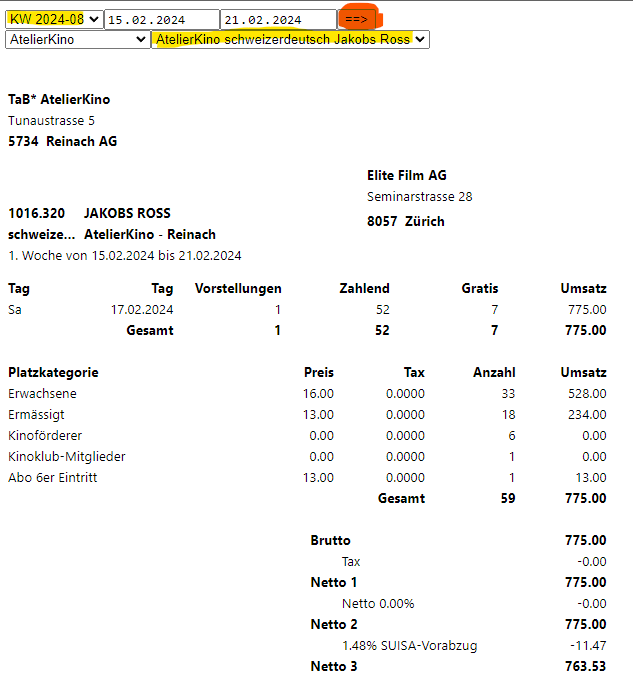
\includegraphics{doc/eintritt.png}

\paragraph{4.1.2 Kiosk}\label{kiosk}

\hyperref[Inhaltsverzeichnis]{Inhaltsverzeichnis}

\textbf{Kiosk 02.12.23.txt}\\
Copy paste von html für jede Vorführung und Speichern unter
``input/advance tickets/Kiosk xx.xx.xx.txt''.\\
Im Menu auf ``DecompteCaisse''
\url{https://www.advance-ticket.ch/decomptecaisse?lang=de} navigieren.\\
Spalte 1 Das Datum muss gewählt werden, Spalte 2 ``reinach'', Splate 3
``Atelierkino Kasse'' und Spalte 4 ``\ldots{}'' eingestellt werden.\\
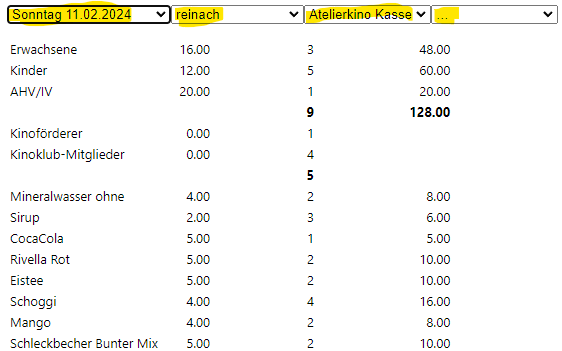
\includegraphics{doc/Kiosk.png}

\paragraph{4.1.3 Shows}\label{shows}

\hyperref[Inhaltsverzeichnis]{Inhaltsverzeichnis}

\textbf{Shows.txt}\\
Copy paste von html für die gewünschte Abrechnungsperiode. Bitte
speichern unter ``input/advance tickets/Shows.txt''\\
Im Menu auf ``Shows'' \url{https://www.advance-ticket.ch/shows?lang=de}
navigieren.\\
Spalte 1 startdatum wählen 1.1.20xx, Spalte 2 Enddatum wählen
31.12.20xx\\
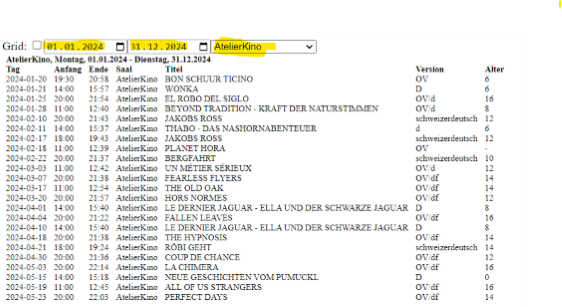
\includegraphics{doc/shows.png}

\subsubsection{4.2 Excel Dateien}\label{excel-dateien}

\hyperref[Inhaltsverzeichnis]{Inhaltsverzeichnis}

Im Verzeichniss \textbf{\ldots/Kinoklub/input/} kann mit Hilfe von
Excelfiles folgendes definiert werden:

\paragraph{4.2.1 Einkaufspreise}\label{einkaufspreise}

\hyperref[Inhaltsverzeichnis]{Inhaltsverzeichnis}

Die Einkaufspreise die ab einem bestimmten Datum gültig sind. ``Einkauf
Kiosk xx.xx.xx.xlsx''\\
Die Einkaufspreise für die Kioskverkäufe müssen gepflegt werden. Ändern
sich die Einkaufspreise so muss ein neues File mit neuerem gültigkeis
Datum erstellt werden.\\

\begin{itemize}
\tightlist
\item
  Achtung!\\
  Die alte Dateien dürfen nicht gelöscht werden.
\end{itemize}

\paragraph{4.2.2 Spezialpreise Kiosk}\label{spezialpreise-kiosk}

\hyperref[Inhaltsverzeichnis]{Inhaltsverzeichnis}

In der Datei \textbf{Spezialpreisekiosk.xlsx} müssen die Sonderangebote
(Spez-Verkaufsartikel) definiert werden.\\
Diese Datei wird benötigt um die Spezialpreise

\begin{itemize}
\tightlist
\item
  Spez 1
\item
  Spez 2
\item
  Spez 3
\item
  Spez 4
\end{itemize}

nach zuschlagen.

\paragraph{4.2.3 Verleiherabgaben}\label{verleiherabgaben}

\hyperref[Inhaltsverzeichnis]{Inhaltsverzeichnis}

Die Verleiherabgaben müssen in der Datei
\textbf{\ldots/Kinoklub/input/Verleiherabgaben.xlsx} definiert werden.\\

\begin{itemize}
\item
  Im \textbf{Tab Verleiherabgaben} muss der \textbf{``minimal Abzug''}
  sowie \textbf{``Abzug \%''} oder nur der \textbf{``Abzug fix
  {[}CHF{]}''} definiert werden. ~ Beide Einträge sind nicht erlaubt.
\item
  Im \textbf{Tab Kinoförderer gratis} muss für jeden Verleiher definiert
  werden, ob gewisse Platzkategorien (z.B.Kinoförderer Tickets) als
  gratis abgerechnet werden dürfen.\\
  Wenn \textbf{nein} gewählt wird, dann werden zusätzlich die
  Platzkategorieen welche in \texttt{c\_P\_kat\_verechnen} definiert
  sind, auch als Umsatz verrechnet.\\
  Der Rechnungsbetrag der Verleiherrechnung an den Kinoklub wird demnach
  grösser.
\end{itemize}

\paragraph{4.2.4 Einnahmen und Ausgaben}\label{einnahmen-und-ausgaben}

\hyperref[Inhaltsverzeichnis]{Inhaltsverzeichnis}

Alle Einnahmen und Ausgaben müssen in der Datei
\textbf{\ldots/Kinoklub/input/Einnahmen und Ausgaben.xlsx} definiert
werden.\\
Ja nach \textbf{Ausgabentyp} muss eine \textbf{Kategorie,
(Buchhaltungskonto)} verwendet werden. Das ist nötig um die Einnahmen
und Ausgaben korrekt in den \textbf{Berichten} auszuwerten.

\newpage

\subsection{5 Script Konfiguration}\label{script-konfiguration}

\hyperref[Inhaltsverzeichnis]{Inhaltsverzeichnis}

Die Datei \textbf{``Erstelle Abrechnung.R''} enhält am Anfang die
folgenden definition die abgeändert werden können um das Verhalten des
Scripts zu beeinflussen.

\subsubsection{5.1 Abrechnung für
Filmvorführungen}\label{abrechnung-fuxfcr-filmvorfuxfchrungen}

\hyperref[Inhaltsverzeichnis]{Inhaltsverzeichnis}

\begin{itemize}
\tightlist
\item
  Für jede Filmvorführung eine Abrechnung erstellen.\\
  \texttt{c\_run\_single} \textless- TRUE
\item
  Es werden nur die Jahresabrechnung und die Statistik-Berichte
  erstellt.\\
  \texttt{c\_run\_single} \textless- FALSE
\end{itemize}

\subsubsection{5.2 Inhaltsverzeichnisse}\label{inhaltsverzeichnisse}

\hyperref[Inhaltsverzeichnis]{Inhaltsverzeichnis}

Sollen die erstellten Berichte mit Inhaltsverzeichniss erstellt werden?

\begin{itemize}
\tightlist
\item
  Ja\\
  \texttt{toc} \textless- TRUE
\item
  Nein\\
  \texttt{toc} \textless- FALSE
\end{itemize}

\subsubsection{5.3 Mehrwertsteuersatz}\label{mehrwertsteuersatz}

\hyperref[Inhaltsverzeichnis]{Inhaltsverzeichnis}

c\_MWST \textless- 8.1 \#\%

\subsubsection{5.4 Platzkategorien ohne Umsatz die dennoch abgerechnet
werden
müssen.}\label{platzkategorien-ohne-umsatz-die-dennoch-abgerechnet-werden-muxfcssen.}

\hyperref[Inhaltsverzeichnis]{Inhaltsverzeichnis}

Für gewisse Verleiher müssen zusätzliche Platzkategorieen abgerechnet
werden. Die Defintion findet sich in der Datei ``Verleiherabgaben.xlsx''
TAB ``Kinoförderer gratis''.\\
Die Variable \texttt{df\_P\_kat\_verechnen} definiert welche
Platzkategorien ohne Umsatz zusätzlich verrechnet werden und zu welchem
Preis.\\
\texttt{df\_P\_kat\_verechnen} \textless- tibble(Kinoförderer =
``Kinoförderer'', Verkaufspreis = 13) ~

\subsubsection{5.5 Ausgabeformate}\label{ausgabeformate}

\hyperref[Inhaltsverzeichnis]{Inhaltsverzeichnis}

\begin{itemize}
\tightlist
\item
  \texttt{c\_render\_option} \textless- ``1'' only html
\item
  \texttt{c\_render\_option} \textless- ``2'' only docx
\item
  \texttt{c\_render\_option} \textless- ``3'' only pdf (Achtung für pdf
  install Latex for Windows (Miktex) for Mac (MacTex))
\item
  \texttt{c\_render\_option} \textless- ``4'' html and docx
\item
  \texttt{c\_render\_option} \textless- ``5'' html and pdf (Achtung für
  pdf install Latex for Windows (Miktex) for Mac (MacTex))
\item
  \texttt{c\_render\_option} \textless- ``6'' docx and pdf (Achtung für
  pdf install Latex for Windows (Miktex) for Mac (MacTex))
\item
  \texttt{c\_render\_option} \textless- ``7'' html, docx and pdf
  (Achtung für pdf install Latex for Windows (Miktex) for Mac (MacTex))
\end{itemize}

\newpage

\subsection{6 Ablauf}\label{ablauf}

\hyperref[Inhaltsverzeichnis]{Inhaltsverzeichnis}

``Erstelle Abrechnung.R'' Script führt folgendes auf.

\begin{enumerate}
\def\labelenumi{\arabic{enumi}.}
\tightlist
\item
  Konfigurations variablen erstellen.
\item
  Die Daten werden mit Script ``read and convert.R'' eingelesen und
  Konvertiert. Der Script ``read and convert.R'' benötigt ``function.R''
  und ``Kiosk.R''
\item
  Erstellen Statistikbericht
\item
  Erstellen Jahresbericht
\item
  Erstellen Jahresbericht detailed
\item
  Erstellen Abrechnung Filmvorführung pro Datum respektive Vorführung
\item
  Site-Map mit Berichtvorschau wird erstellt
\item
  Daten für Webserver werden erstellt.
\end{enumerate}

\newpage

\subsection{7 Berichte}\label{berichte}

\hyperref[Inhaltsverzeichnis]{Inhaltsverzeichnis}

Alle Dateien die erzeugt wurden finden sich im
\textbf{\ldots/Kinoklub/output/} Verzeichniss.

\begin{itemize}
\tightlist
\item
  Für jede Filmvorführung respektive Datum wird ein Abrechnung erstellt.
\item
  Es wird eine Jahresbarechnung und eine detalierte Jahresabrechnung
  erstellt.
\item
  Es wird eine Statistik mit Porgnosen erstellt.
\item
  Alle verwendeten Datensätze werden in ein Excelfile abgespeichert.
\end{itemize}

\subsubsection{7.1 Abrechnung
Filmvorführung}\label{abrechnung-filmvorfuxfchrung}

\hyperref[Inhaltsverzeichnis]{Inhaltsverzeichnis}

Es wird eine Filmabrechnung pro Event (Datum) erstellt.

\begin{itemize}
\tightlist
\item
  Übericht\\
\item
  Filmvorführung

  \begin{itemize}
  \tightlist
  \item
    Kino Besucherzahlen und Umsatz

    \begin{itemize}
    \item
      Filmabgaben\\
    \item
      Verleiherrechnung\\
      In der Datei \textbf{``\ldots/Kinoklub/input/Einnahmen und
      Ausgaben.xlsx''} in den \textbf{Ausgaben}\\
      wird die Kategorie \textbf{Verleiher} berücksichtigt.
    \item
      Prozentualle Abgaben\\
      Der Suisaabzug wird vom Umsatz berechnet.\\

      In der Datei
      \textbf{``\ldots/Kinoklub/input/Verleiherabgaben.xlsx''} sind
      \textbf{Abzug \%}, \textbf{Minimal Abzug} oder \textbf{Abzug fix
      {[}CHF{]}} definiert.\\

      \begin{enumerate}
      \def\labelenumi{\arabic{enumi}.}
      \tightlist
      \item
        Fall:\\
        \textbf{Netto3} x \textbf{Abzug \%} \textgreater{}
        \textbf{Minimal Abzug}\\
        Verleiherabzug: \textbf{Netto3} x \textbf{Abzug \%}
      \item
        Fall:\\
        \textbf{Netto3} x \textbf{Abzug \%} \textless{} \textbf{Minimal
        Abzug}\\
        Verleiherabzug: \textbf{Minimal Abzug}\\
      \item
        Fall:\\
        \textbf{Abzug fix {[}CHF{]}}\\
        Verleiherabzug: \textbf{Abzug fix {[}CHF{]}}
      \end{enumerate}
    \item
      Reklamematerial und Porto\\
      Das \textbf{Reklamematerial und Porto} werden aus der Differenz
      der \textbf{Verleiherrechnung} und den \textbf{Prozentualle
      Abgaben} berechnet.
    \item
      MWST auf Verleiherrechnung\\

      \begin{enumerate}
      \def\labelenumi{\arabic{enumi}.}
      \tightlist
      \item
        Fall: Vereiherrechnung vorhanden\\
        MWST wird mit der Verleiherrechnung berechnet.
      \item
        Fall: Vereiherrechnung nicht vorhanden\\
        MWST wird aus dem Umsatz berechnet.\\
      \end{enumerate}
    \end{itemize}
  \item
    Gewinn / Verlust aus Tickerverkauf\\
    Der Gewinn/Verlust wird aus \textbf{Umsatz} -
    (\textbf{Suisa-Abzug}+\textbf{Verleiherabzug}+\textbf{MWST}+\textbf{Reklamematerial
    und Porto})
  \end{itemize}
\item
  Event

  \begin{itemize}
  \tightlist
  \item
    Einnahmen

    \begin{itemize}
    \tightlist
    \item
      In der Datei \textbf{``\ldots/Kinoklub/input/Einnahmen und
      Ausgaben.xlsx''} in den \textbf{Ausgaben}\\
      wird die Kategorie \textbf{Vermietung} wird pro Filmabrechnung
      (Datum) berücksichtigt.
    \end{itemize}
  \item
    Ausgaben

    \begin{itemize}
    \tightlist
    \item
      In der Datei \textbf{``\ldots/Kinoklub/input/Einnahmen und
      Ausgaben.xlsx''} in den \textbf{Ausgaben}\\
      wird die \textbf{Eventausgaben} wird pro Filmabrechnung
      (Spieldatum) berücksichtigt.
    \end{itemize}
  \end{itemize}
\item
  Kiosk

  \begin{itemize}
  \tightlist
  \item
    Gewinn pro Artikel\\
    In der Datei \textbf{``\ldots/Kinoklub/input/Einkauf Kiosk
    xx.xxx.xx.xlsx''}~ist der Gewinn pro Artikel definiert.
  \item
    Umsatz Für den Verkaufsartikel gibte es keine Definition in der
    Datei \textbf{``\ldots/Kinoklub/input/Einkauf Kiosk
    xx.xxx.xx.xlsx''}\\
  \item
    Einnahmen\\
    Die Einnahmen werden aus Gewinn pro Artikel und dem Umsatz für
    Spezialpreise berechnet.
  \item
    Ausgaben\\
    Achtung!\\
    Für Verkaufsartikel ohne Lieferant müssen Eventausgaben definiert
    werden.
  \end{itemize}
\item
  Kioskumsatz pro Gast

  \begin{itemize}
  \tightlist
  \item
    Kioskumsatz aller Gäste
  \item
    Kioskumsatz pro zahlender Gast
  \end{itemize}
\item
  Kasse\\
  Die Kioskkasse wird auch für Barauszahlung von stornierten Tickets
  genutzt.
\item
  Gewinn / Verlust\\
  Summe aus Einnahmen und Ausgaben
\end{itemize}

\subsubsection{7.2 Jahresabrechnungen}\label{jahresabrechnungen}

\hyperref[Inhaltsverzeichnis]{Inhaltsverzeichnis}

Die Einnahmen und Ausgaben werden für die Jahresabrechnung verwendet und
je nach Kategorie der Rechnung zugewiesen. Die folgenden Kategorien
werden in den Jahresrechnungen separat behandelt.

\begin{itemize}
\tightlist
\item
  Filmvorführungen\\

  \begin{itemize}
  \tightlist
  \item
    Eintritt

    \begin{itemize}
    \tightlist
    \item
      Einnahmen Ticketverkauf
    \item
      Abgaben Ticketverkauf

      \begin{itemize}
      \tightlist
      \item
        Suisaabgaben
      \item
        Verleiherabgaben
      \item
        Nebenkosten
      \item
        MWST auf Verleiherleistungen
      \end{itemize}
    \end{itemize}
  \end{itemize}
\item
  Event

  \begin{itemize}
  \tightlist
  \item
    Eventeinnahmen\\
    Einnahmen für den Event, z.B. Beiträgemitveranstalter,
    Eventsponsoring, \ldots{}
  \item
    Eventausgaben\\
    Alle Ausgaben die für den Event, z.B. Werbung, Esswaren, Spesen,
    \ldots{}
  \end{itemize}
\item
  Kiosk

  \begin{itemize}
  \tightlist
  \item
    Einnahmen\\
    Die Einnahmen werden mit \textbf{``Anzahl x Verkaufspeis für
    Verkaufsartikel''} berechnet.
  \item
    Ausgaben

    \begin{itemize}
    \tightlist
    \item
      Einkauf Getränke\\
      Die Getränke werden von Theater am Bahnhof eingekauft.\\
      Falls in der Datei \textbf{\ldots/Kinoklub/input/Einkauf Kiosk
      xx.xx.xx.xlsx} der Lieferant \textbf{``Schüwo''} definiert wurde
      wird der Verkaufsartikel als Getränk ausgegeben.\\
      Der Getränkeeinkauf wird mit \textbf{``Anzahl x Einkaufspreis''}
      berechnet.
    \item
      Einkauf Kino\\
      Für alle Verkaufsartikel mit Ausnahme der Getränke wird in der
      Datei \textbf{``\ldots/Kinoklub/input/Einnahmen und
      Ausgaben.xlsx''} ~ mit Kategorie \textbf{Kiosk} definiert.
    \end{itemize}
  \end{itemize}
\item
  Abos / Kinogutscheine

  \begin{itemize}
  \tightlist
  \item
    Einnahmen

    \begin{itemize}
    \tightlist
    \item
      Abos
    \item
      Kinogutscheine
    \item
      Summe
    \end{itemize}
  \item
    Eingelöst

    \begin{itemize}
    \tightlist
    \item
      Abos
    \item
      Kinogutscheine
    \end{itemize}
  \item
    Kurzfristiges zinsloses Fremd-Kapital
  \end{itemize}
\item
  Vermietung\\

  \begin{itemize}
  \tightlist
  \item
    Einnahmen\\
    Vermietung Kinosaal, Beiträge von mit Veranstallter, \ldots{}
  \item
    Ausgaben\\
    Mietkosten für Filme und Material, \ldots{}
  \end{itemize}
\item
  Werbung

  \begin{itemize}
  \tightlist
  \item
    Einnahmen\\
    Die Werbeeinnahme aus Kinowerbung druch Trailers, Dias für
    Sponsoren, \ldots{}
  \item
    Ausgaben\\
    Inserate, Drucksachen, Homepage, \ldots{}
  \end{itemize}
\item
  Personalaufwand\\
  Löhne
\item
  Sonstiges

  \begin{itemize}
  \tightlist
  \item
    Einnahmen\\
    Sponsoen, Gönner, Kulturbeiträge, \ldots{}
  \item
    Ausgaben\\
    Kinomiete an Theater am Bahnhof AG, Mitgliederbeiträge, Ciné
    Bulletin, \ldots{}
  \end{itemize}
\end{itemize}

\subsubsection{7.3 Statistik}\label{statistik}

\hyperref[Inhaltsverzeichnis]{Inhaltsverzeichnis}

\begin{itemize}
\tightlist
\item
  Gewinn/Verlust

  \begin{itemize}
  \tightlist
  \item
    Prognose\\
    Die Prognose wird mit der Kumuliertensumme pro Datum als lineares
    Model erstellt.
  \end{itemize}
\item
  Ticketverkauf

  \begin{itemize}
  \tightlist
  \item
    Prognose\\
    Die Prognose wird mit der Kumuliertensumme pro Datum als lineares
    Model erstellt.
  \item
    Eintritte

    \begin{itemize}
    \tightlist
    \item
      Anzahl\\
      Diagramm
    \item
      Umsatz

      \begin{itemize}
      \tightlist
      \item
        Prognose\\
        Die Prognose wird mit der Kumuliertensumme pro Datum als
        lineares Model erstellt.
      \end{itemize}
    \end{itemize}
  \item
    Filmabgaben

    \begin{itemize}
    \tightlist
    \item
      Prognose\\
      Die Prognose wird mit der Kumuliertensumme pro Datum als lineares
      Model erstellt.
    \end{itemize}
  \end{itemize}
\item
  Abos

  \begin{itemize}
  \tightlist
  \item
    Einnahmen
  \item
    Eingelöst
  \item
    Kredit
  \end{itemize}
\item
  Kiosk-Gewinn pro Vorführung

  \begin{itemize}
  \tightlist
  \item
    Prognose\\
    Die Prognose wird mit der Kumuliertensumme pro Datum als lineares
    Model erstellt.
  \end{itemize}
\item
  Kiosk

  \begin{itemize}
  \tightlist
  \item
    Verkaufsartikel
  \item
    Ladenhüter (keine Verkäufe)
  \item
    Kiosk Umsatz pro Gast

    \begin{itemize}
    \tightlist
    \item
      Prognose\\
      Die Prognose wird mit der Kumuliertensumme pro Datum als lineares
      Model erstellt.
    \end{itemize}
  \item
    Umsatz pro zahlender Gast

    \begin{itemize}
    \tightlist
    \item
      Prognose\\
      Die Prognose wird mit der Kumuliertensumme pro Datum als lineares
      Model erstellt.
    \end{itemize}
  \end{itemize}
\end{itemize}

\subsubsection{7.4 Daten als Excel-Datei}\label{daten-als-excel-datei}

\hyperref[Inhaltsverzeichnis]{Inhaltsverzeichnis}

Die Eingelesenen und verarbeiteten Datensätze werden in einen
Excel-Datei gespeichert.\\

\begin{verbatim}
.../Kinoklub/output/Auswertung.xlsx
\end{verbatim}

\newpage

\subsection{8 Versionshistorie}\label{versionshistorie}

\hyperref[Inhaltsverzeichnis]{Inhaltsverzeichnis}

2024 V1.0 Go Live mit Stefan Jablonski, Nadia und Florian Wagner\\
2024 V1.1 Verkauf von Abos und Gutscheinen wird in der Jahresabarechnung
berücksichtigt\\
2024 V1.2 Abrechnung für Kinowerbung
hinzugefügt:\ldots./output/Auswertung.xlsx und Prognosen in der
Statistik überarbeitet\\
2024 V1.3 Neuer Bericht Statistik\_DT hinzugefügt. Interaktives
durchsuchen aller Tabellen\\

\end{document}
